\section{Visual Feature Examples on Natural Images}
\label{sec:visual-examples}
The digit benchmark establishes an executable protocol, but it provides
only a narrow view of visual features. We now examine a pretrained image
encoder on animals and vehicles. Following the investigative approach of
\emph{Zoom In}~\cite{olah2020zoom}, we combine highly activating dataset
examples, spatial response maps, and explicit comparisons between feature
requirements. These are newly computed figures, not reproductions of
Distill's images or evidence for its InceptionV1 circuits.

\subsection{A fixed encoder and an inspectable sample}
\label{sub:natural-protocol}
We use ResNet34~\cite{he2016resnet} with torchvision's
\texttt{IMAGENET1K\_V1} weights~\cite{torchvisionResnet34} and CIFAR-10
\cite{krizhevsky2009}. For each of the ten CIFAR-10 classes, take the
first 125 images in the official training order and the first 25 in the
official test order. The first 100 selected training images per class
train the surrogate; the remaining 25 form a reserved calibration set.
Thus there are 1,000 training, 250 calibration, and 250 test images.
The examples below use fixed rules and do not tune on the reserved
calibration set. This deterministic subset is illustrative, not a
representative random sample of all natural images.

Each $32\times32$ RGB image is resized bilinearly to $96\times96$ and
normalized using the ImageNet channel means and standard deviations.
The smaller resolution is a declared departure from the weight package's
standard evaluation transform, chosen to keep extraction inexpensive.
We cache the output of the complete third residual stage, after its
last addition and ReLU: a $6\times6$ grid of 256-dimensional activations.
The backbone remains frozen and its ImageNet classifier is not evaluated
as a CIFAR-10 classifier.

Each channel is divided by its root mean square on training sites,
floored at $10^{-6}$. A 256-to-512-to-256 Top-16 SAE is trained on these
scaled activations for 12 epochs with Adam, learning rate 0.001, batch
size 512, and seed 2026. Decoder columns are normalized after each update.
The reconstruction is rescaled to the original channel units before
computing \cref{eq:reconstruction-statistic}. Test reconstruction gives
$R^{2}_{\mathrm{tr}}=0.576$, and 165 of the 512 latent coordinates are
active on training data. This moderate fidelity and substantial inactive
fraction limit the interpretability claim; the experiment is not a
comparison of optimized surrogate architectures.

\subsection{Feature galleries and response profiles}
\label{sub:feature-galleries}
For a class $c$, select a coordinate by its training contrast
\begin{equation}\label{eq:feature-contrast}
 a_{c,j}=
 \frac{\operatorname{mean}_{x\in X_{\mathrm{tr}},\ y_{x}=c}u_{x,j}
       -\operatorname{mean}_{x\in X_{\mathrm{tr}},\ y_{x}\ne c}u_{x,j}}
      {\max(\operatorname{std}_{x\in X_{\mathrm{tr}}}u_{x,j},10^{-12})}.
\end{equation}
Here $y_{x}$ is the dataset class and the standard deviation uses divisor
$|X_{\mathrm{tr}}|$. Process bird, cat, dog, horse, ship, and truck in that
order, taking the highest-contrast coordinate not selected previously;
break ties by coordinate index. This selects coordinates 271, 425, 150,
358, 78, and 461. The class names describe the selection criterion, not
established meanings of the coordinates.

For each selected coordinate, \cref{fig:animal-features,fig:vehicle-features}
show its three highest-activating test images across \emph{all} classes,
paired with the unpooled $6\times6$ code maps. A common color range within
each row permits comparison between its examples: black denotes zero,
and brighter colors denote larger activations. Labels and original
CIFAR test indices make mismatches inspectable. The low-resolution images
are displayed without invented detail. Site maps are response locations
in the feature grid, not segmentation masks or causal attribution maps:
the residual network's receptive fields can cover most or all of an image.

\begin{figure}[p]
 \centering
 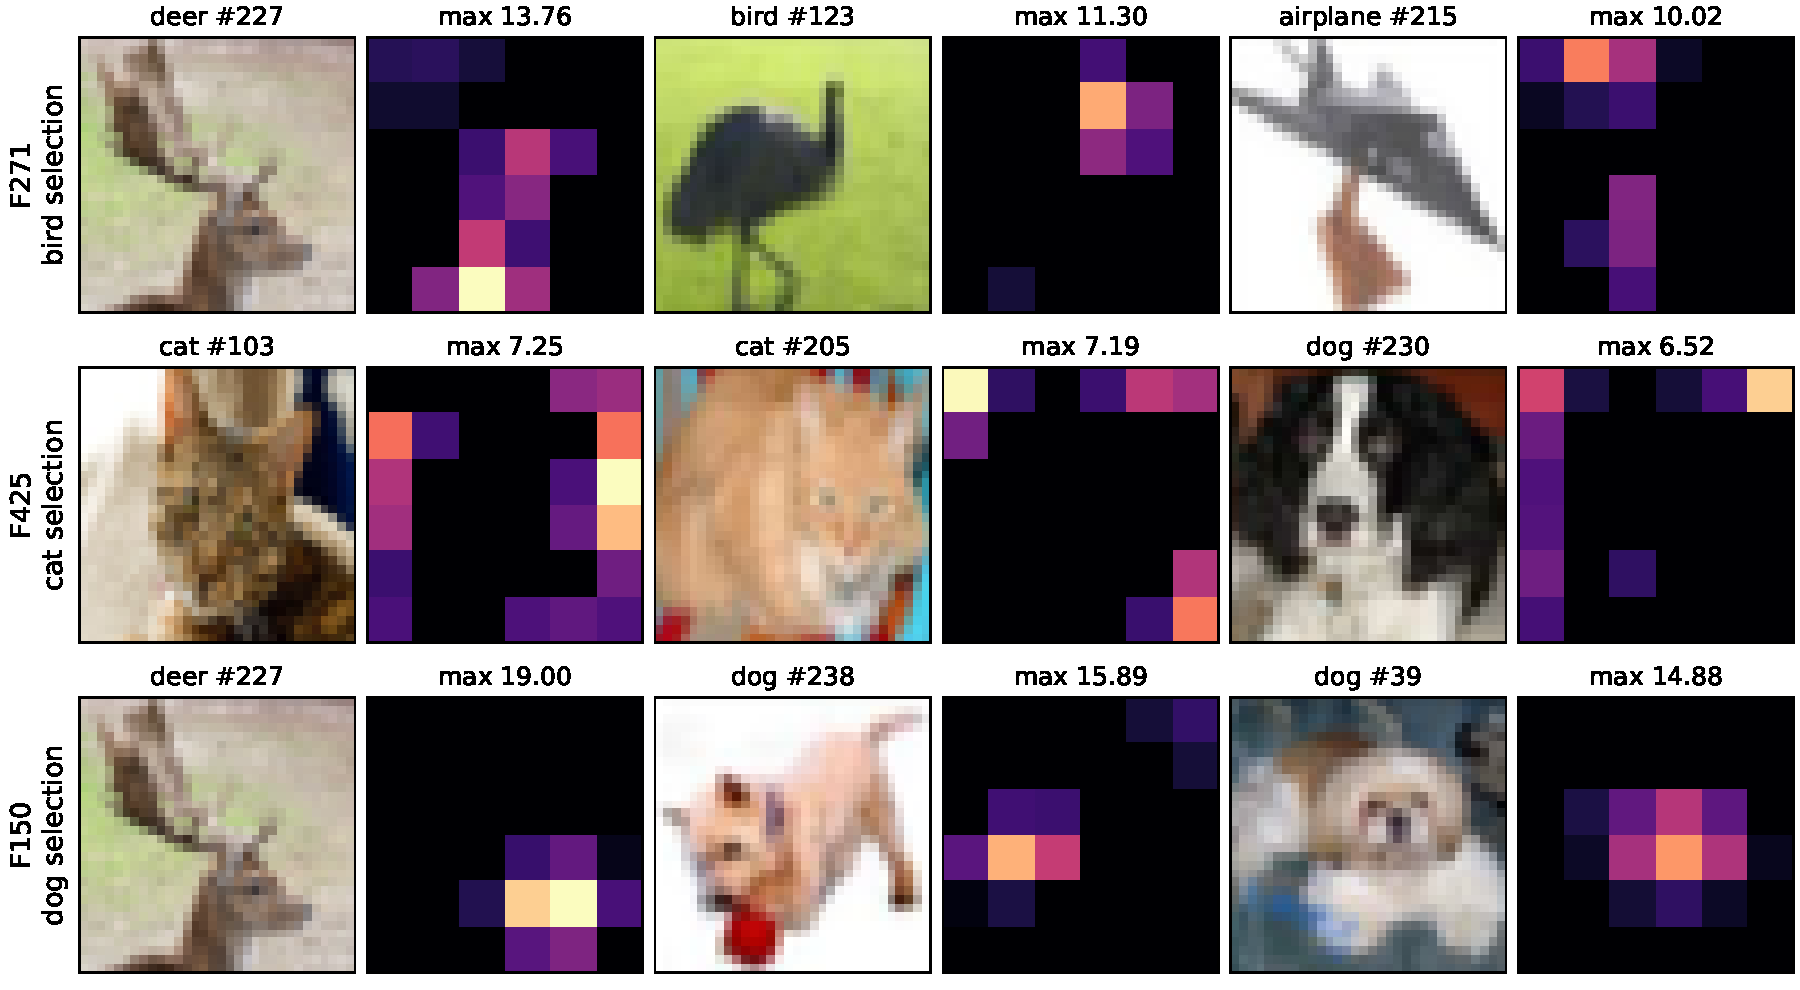
\includegraphics[width=\linewidth]{figures/feature_animals_codexgen.pdf}
 \caption{Dataset exemplars and site activation maps for coordinates
 selected by bird, cat, and dog training contrasts. Each image is followed
 by its measured $6\times6$ feature map; intensity uses a shared scale
 within a row. Titles identify the actual test label, original index,
 and maximum activation. A selected class does not determine the labels
 of the highest-activating examples.}
 \label{fig:animal-features}
\end{figure}

\begin{figure}[p]
 \centering
 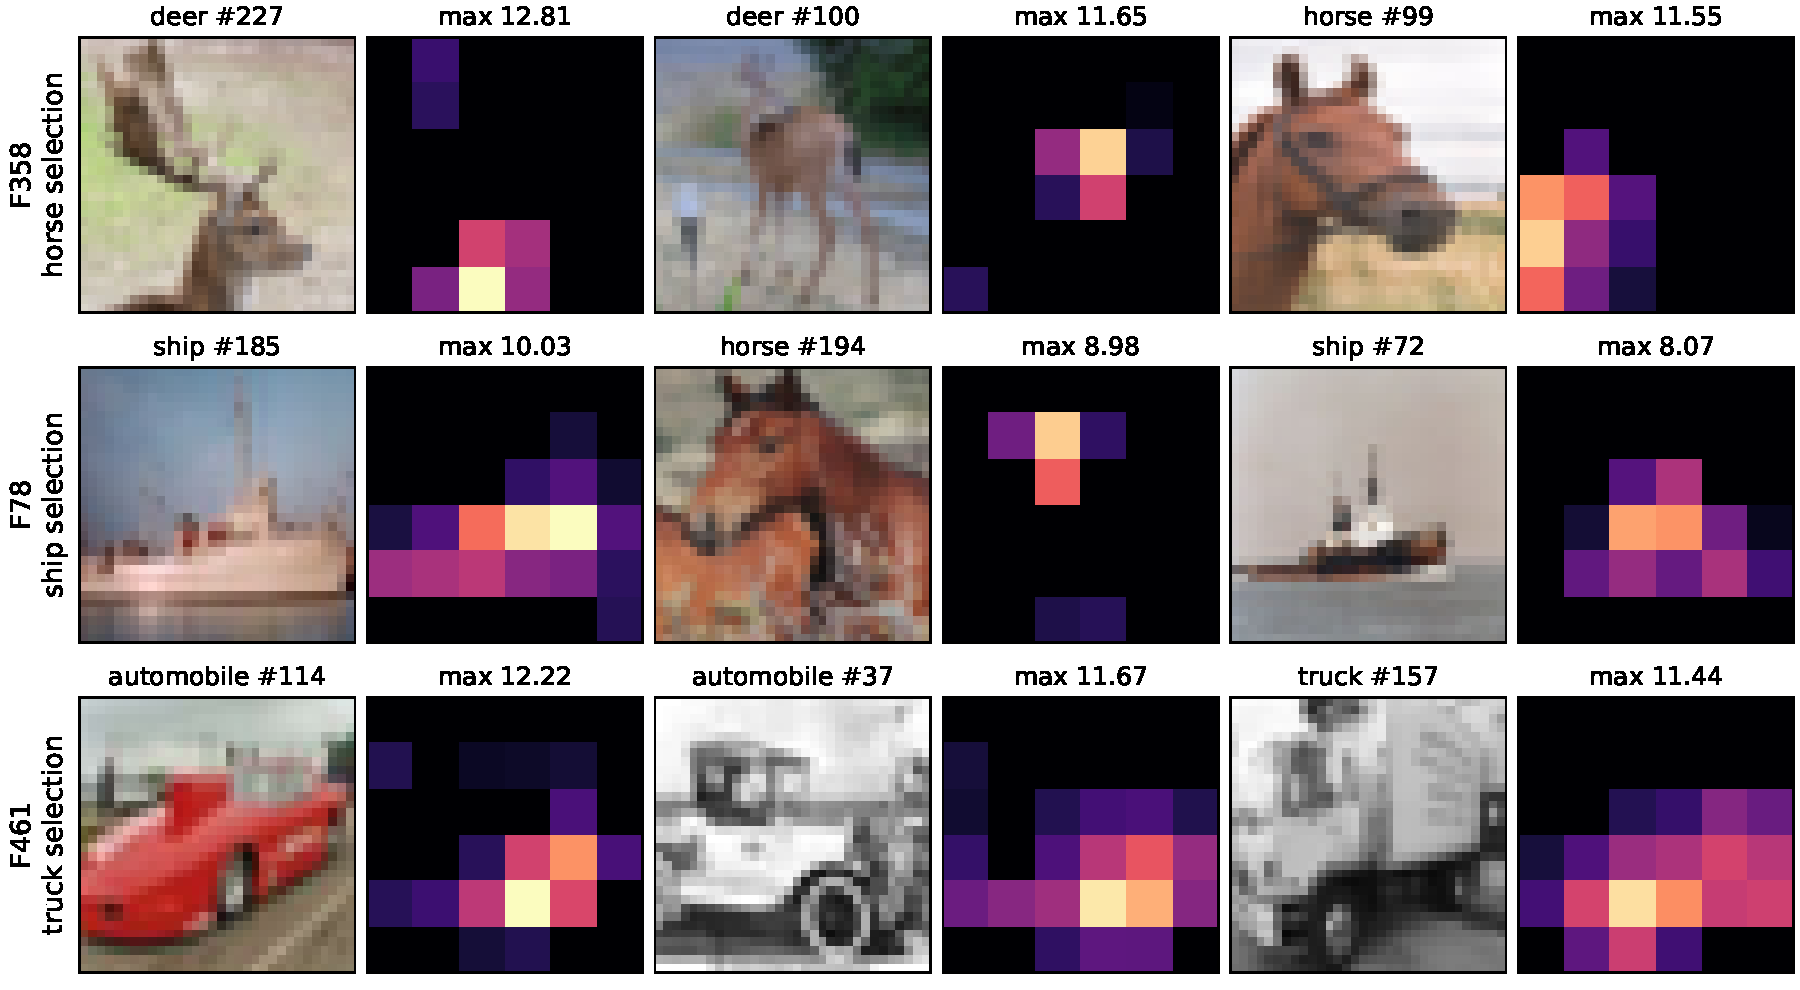
\includegraphics[width=\linewidth]{figures/feature_transport_codexgen.pdf}
 \caption{The same analysis for horse-, ship-, and truck-associated
 coordinates. Deer occur among the strongest horse-associated responses,
 and automobiles among the strongest truck-associated responses. Such
 overlap motivates inspecting feature combinations rather than assigning
 a class meaning from a few favorable examples.}
 \label{fig:vehicle-features}
\end{figure}

\Cref{fig:feature-tuning} summarizes the entire 250-image test sample.
Each cell is the mean max-pooled activation for one class, divided by
the coordinate's training-image root mean square. It is a class response
profile, not a controlled stimulus-tuning experiment. The single-feature
test AP values for the six selected classes are respectively 0.176,
0.338, 0.456, 0.366, 0.451, and 0.514. Equal class prevalence is 0.1.
These descriptive associations neither imply class exclusivity nor show
that a coordinate causes the backbone's prediction.

\begin{figure}[tbp]
 \centering
 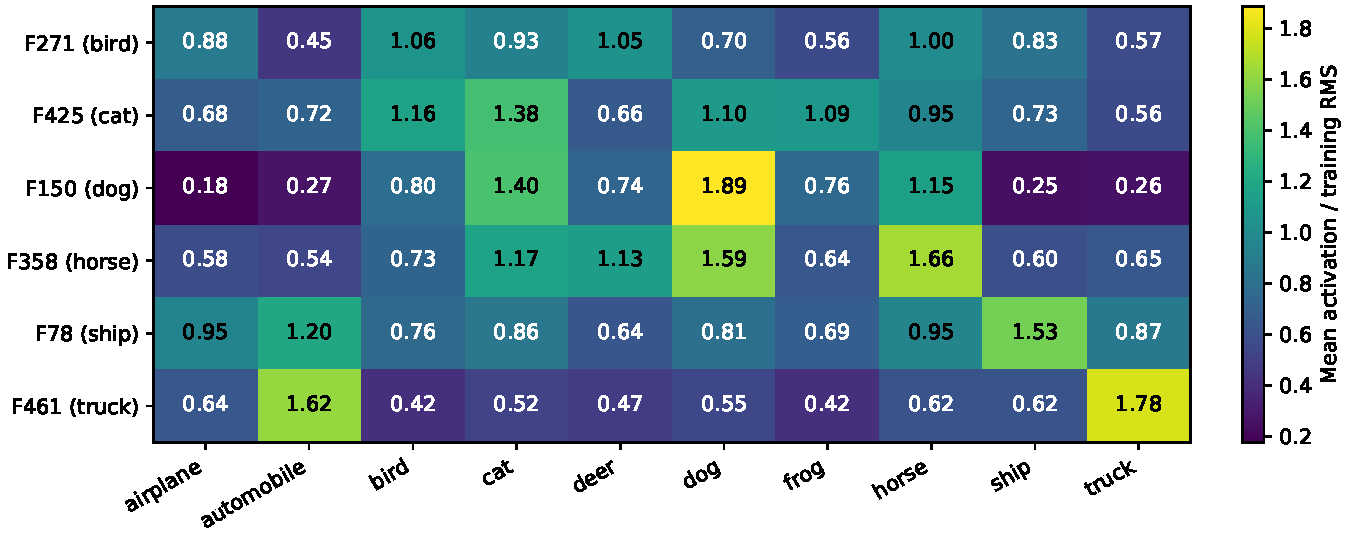
\includegraphics[width=\linewidth]{figures/feature_tuning_codexgen.pdf}
 \caption{Measured class response profiles for all test images, in
 training RMS units. Selection uses training labels; all plotted means
 use the separate test images. Broad and overlapping responses remain
 visible rather than being removed from the gallery.}
 \label{fig:feature-tuning}
\end{figure}

\subsection{Animal and vehicle queries under meet and join}
\label{sub:natural-queries}
To parallel the companion paper's comparisons of related examples, fix
two pairs of associated classes: cat/dog and ship/truck. For each class,
choose the training image with maximal activation of its selected
coordinate, breaking ties by the stored sample order. Keep the two
coordinates selected for that pair. The source query retains half of
each corresponding source-image activation and is zero elsewhere.
Thus both queries use the same coordinate set, even when a source is
selected for only one of its coordinates. The multiplier $0.5$ is fixed,
not selected using test performance. Displayed thresholds are rounded;
counts use the full-precision values saved in the retrieval arrays.

\Cref{fig:animal-queries} shows the cat/dog queries on coordinates
425 and 150. Their test extents contain 40 and 25 images; the meet
retrieves 74 and the join 17. The join extent is exactly the intersection
of the two source extents. All four same-site extents are empty. Hence
these apparent combinations of animal-associated evidence rely on
separate spatial witnesses at the chosen thresholds.

\begin{figure}[p]
 \centering
 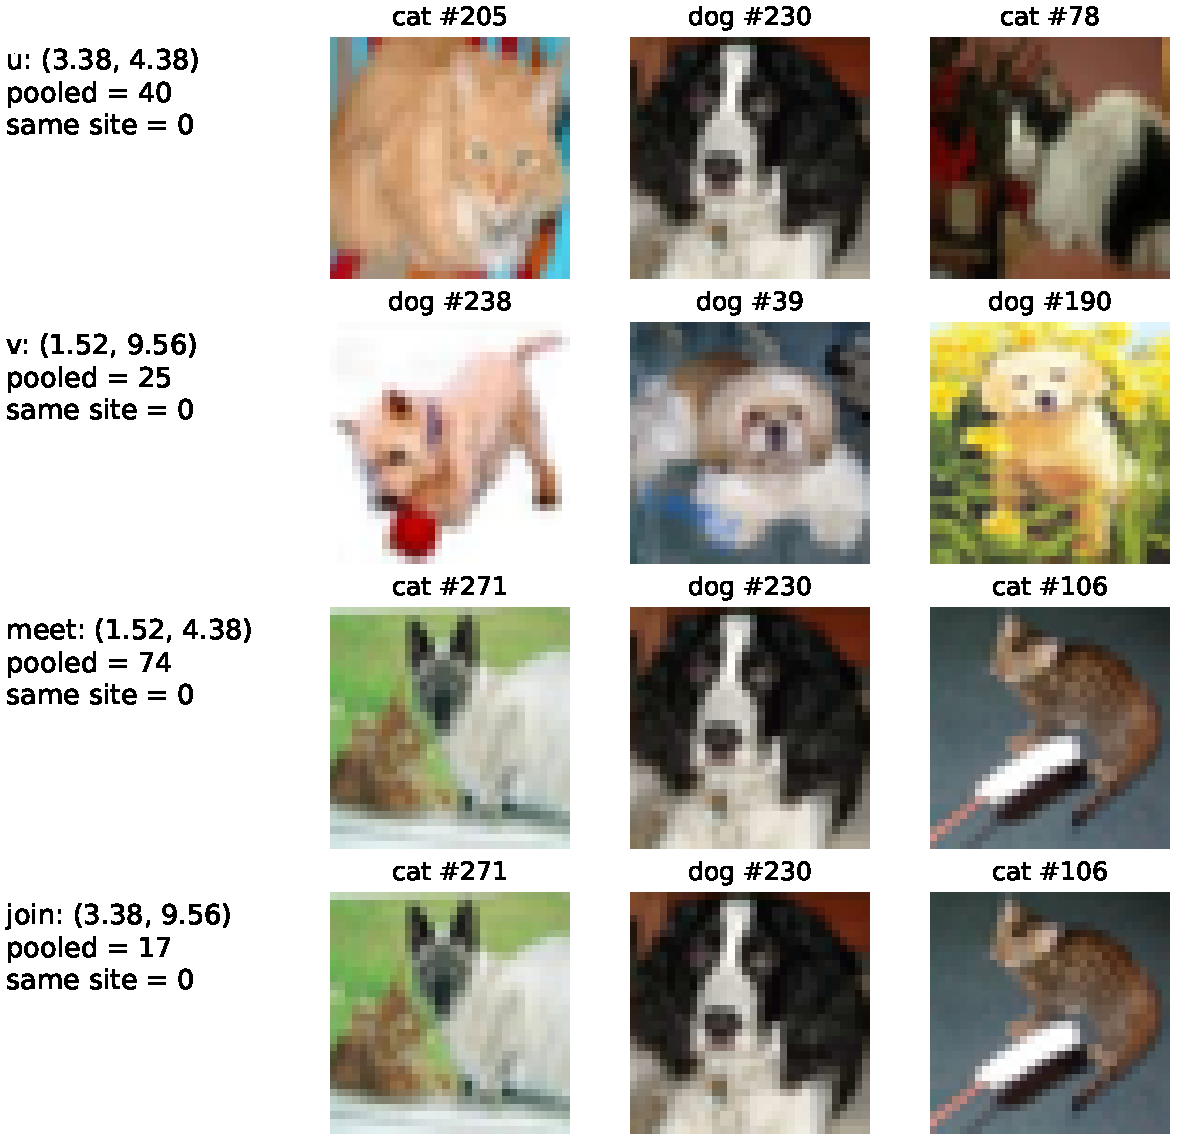
\includegraphics[width=0.9\linewidth]{figures/query_cat_dog_codexgen.pdf}
 \caption{Cat/dog-associated queries, their meet, and their join.
 Thresholds are displayed in coordinate order $(425,150)$. Counts include
 all 250 test images. Each row shows up to three matching images ranked
 by \cref{eq:graded-score}; numbers beside the images are original test
 indices. All four same-site counts are zero.}
 \label{fig:animal-queries}
\end{figure}

For ship/truck-associated coordinates 78 and 461, the source extents
contain 10 and 23 images, the meet contains 158, and the join contains
one automobile image. Their respective same-site counts are 2, 7, 72,
and 0. The sole join match is therefore not an image labeled both ship
and truck, and it has no common spatial witness. The algebra combines
activation requirements; its result is not a conjunction of class names.

\begin{figure}[p]
 \centering
 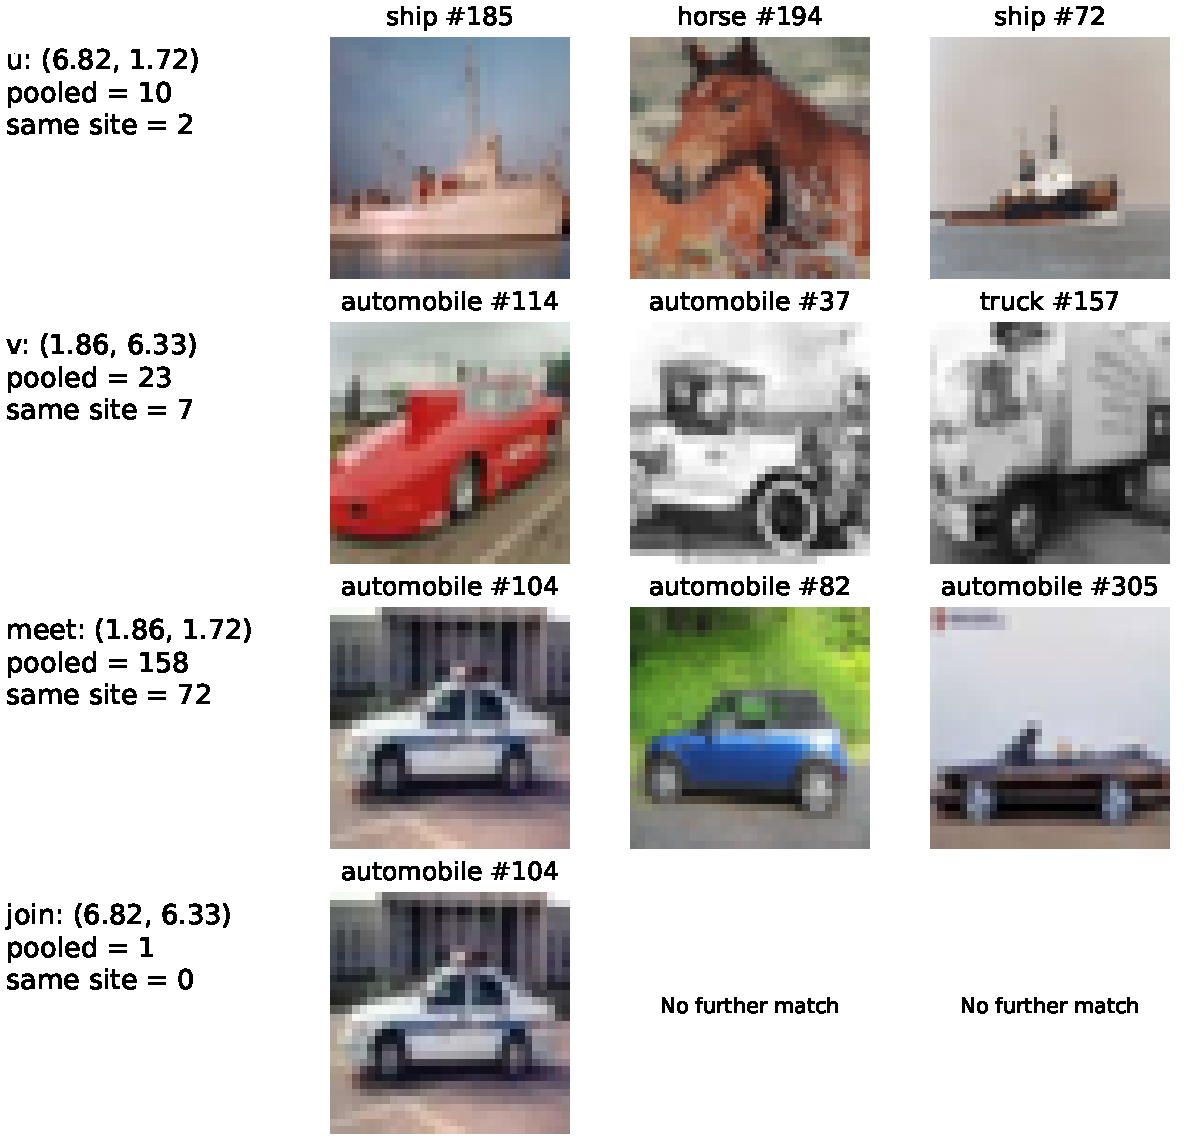
\includegraphics[width=0.9\linewidth]{figures/query_ship_truck_codexgen.pdf}
 \caption{Ship/truck-associated queries on coordinates $(78,461)$.
 The meet is broad, while the join has one pooled match, labeled
 automobile. Its same-site extent is empty. Blank retrieval positions
 explicitly indicate that no further image satisfies the query.}
 \label{fig:vehicle-queries}
\end{figure}

These examples make the semantics of pooling and lattice operations
visible in actual images. Named-city, geographic, or sports-team studies
would require suitable image labels and controls for landmarks, text,
logos, and backgrounds. The present animal and vehicle labels support
the reported comparisons only. Following the distinction between feature
hypotheses and circuit evidence in~\cite{olah2020zoom}, a future causal
analysis should test predictions under controlled interventions rather
than treating these galleries as recovered computational circuits.

\clearpage
